\documentclass[a4paper, 12pt]{article}

\usepackage[warn]{mathtext} % Русский текст в формулах

\usepackage{tablefootnote}  % Cноски для таблиц

%Абзацный отступ

\usepackage{indentfirst}

%Рисунки

\usepackage{graphicx}
\usepackage{wrapfig}

%Гиперссылки и работа с цветом

\usepackage{hyperref}
\usepackage[rgb]{xcolor}
\hypersetup{			%Гиперссылки
	colorlinks=true, 	%false: ссылки в рамках
	urlcolor=blue		%на URL
}

%Русский язык

\usepackage[T2A]{fontenc}		%кодировка
\usepackage[utf8]{inputenc}		%кодировка исходного текста
\usepackage[english, russian]{babel}	%локализация и переносы


%Математика

\usepackage{amsmath, amsfonts, amssymb, amsthm, mathtools, mathrsfs}

%Пакет с градусом

\usepackage{gensymb}

%subfloat
\usepackage{subfig}

\author{Штрайх Роберт}
\title{Работа 4.7.2. Эффект Поккельса}
\date{24 апреля 2022 г.}

\begin{document}
\begin{titlepage}
	\centering
	\vspace{5cm}
	{\scshape\LARGE Московский физико-технический институт \par}
	\vspace{4cm}
	{\scshape\Large Лабораторная работа №4.7.2 \par}
	\vspace{1cm}
	{\huge\bfseries Эффект Поккельса\par}
	\vspace{1cm}
	\vfill
\begin{flushright}
  {\Large выполнили студенты 006 и 007 групп ФЭФМ}\par
	\vspace{0.3cm}
	{\Large Штрайх Роберт}\par
	\vspace{0.3cm}
	{\Large Петрова Софья}\par
\end{flushright}


	\vfill

% Bottom of the page
	Долгопрудный, 2022 г.
\end{titlepage}

\newpage

\textbf{Цель работы:} исследовать интерференцию рассеянного света, прошедшего кристалл; наблюдать изменение характера поляризации света при наложении на кристалл электрического поля.

\textbf{В работе используются:} гелий-неоновый лазер, поляризатор, кристалл ниобата лития, матовая пластинка, экран, источник высоковольтного переменного и постоянного напряжения, фотодиод, осциллограф, линейка.

\section{Теоретические сведения}

\textit{Эффект Поккельса} -- изменение показателя преломления света в кристалле под действием электрического поля.

Рассмотрим кристалл ниобата лития: его оптические свойства обладают симметрией вращения относительно выделенного направления - оптической оси $Z$. Для волны, распространяющейся вдоль $Z$, показатель преломления равен $n_e$, а для волны, перпендикулярной оптической оси, -- $n_o$, причем $n_o > n_e$. Волну длины $\lambda = 2\pi/k$, проходящую под углом $\theta$ к оси $Z$ в кристалле, принято раскладывать на обыкновенную и необыкновенную. Для вектора напряженности обыкновенной волны верно: $\mathbf{E_o} \perp (\mathbf{k}, \mathbf{e_z})$, -- и показатель преломления $n_1 = n_o$. Для вектора напряженности необыкновенной: $\mathbf{E_e} \in (\mathbf{k}, \mathbf{e_z})$, и показатель преломления $n_2$ зависит от $\theta$ по закону:

	\[ \frac{1}{n_2^2} = \frac{\cos^2\theta}{n_o^2} + \frac{\sin^2\theta}{n_e^2} \]

	Разность хода обыкновенной и необыкновенной волн при прохождении кристалла длиной $l$ составляет:

	\[ \Delta = kl(n_1 - n_2) = \frac{2\pi}{\lambda} \cdot l (n_1 - n_2) \]

	С учетом зависимости $n_2(\theta)$ для малых углов $\theta$ в приближении $n_o \approx n_e$:

	\begin{equation}
		\Delta = \frac{2\pi}{\lambda}\cdot l (n_o - n_e)\theta^2
	\end{equation}

\clearpage
		\begin{figure}[h!]
			\centering
		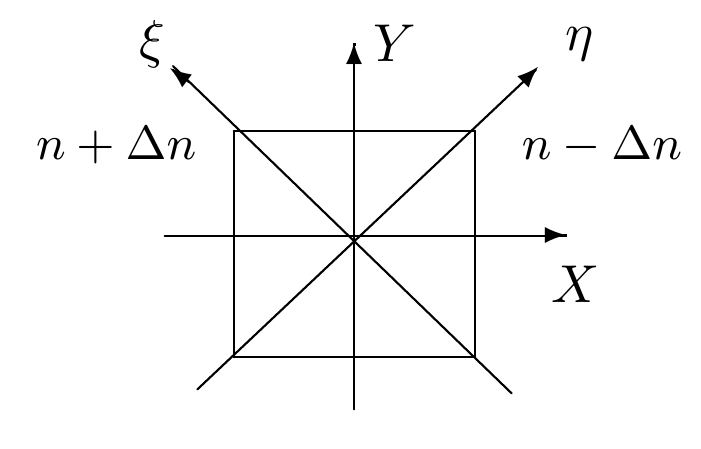
\includegraphics[width=0.6\linewidth]{pokkels.png}
		\caption{Эффект Поккельса: главные направления при наложении электрического поля}
		\label{pokkels}
	\end{figure}


	Направления постоянной разности фаз задают косинусы $\cos\theta$, следовательно, интерференционная картина являет концентрические окружности.

	Поместим кристалл ниобата лития в постоянное электрическое поле $E_{эл}$, направленное по оси $X$, перпендикулярной оптической оси $Z$. В плоскости $(X,Y)$ возникают быстрая и медленная оси под углами $45^\circ$ к $X$, $Y$, соответствующие показателям преломления $(n_o - \Delta n)$ и $(n_o + \Delta n)$, здесь $\Delta n = A\cdot E_{эл}$, $A$ -- константа, зависящая от свойств материала.

	Появление главных направлений $\xi$ и $\eta$ иллюстрирует рисунок \ref{pokkels}.


\section{Экспериментальная установка}


\begin{figure}[h!]
\begin{center}
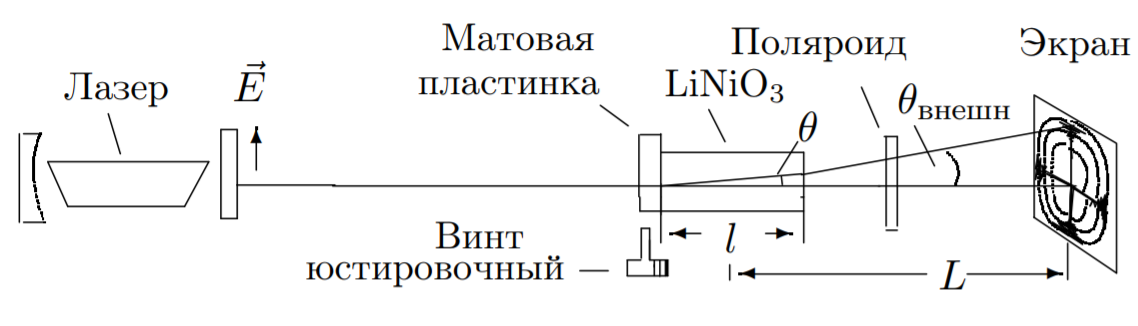
\includegraphics[width = 0.8\textwidth]{1.png}
\end{center}
\caption{Схема для наблюдения интерфереционной картины}
\label{scheme_watch}
\end{figure}

Если перед кристаллом, помещённым между поляроидами, расположить линзу или матовую пластинку, то на экране за поляроидом мы увидим тёмные концентрические окружности -- результат интерференции обыкновенной и необыкновенной волн. При повороте выходного поляроида на $90^\circ$ картина меняется с позитива на негатив (на месте светлых пятен тёмные и наоборот). В случае, когда разрешённое направление анализатора перпендикулярно поляризации лазерного излучения, радиус тёмного кольца с номером $m$ равен
\begin{equation}
r_m^2 = \dfrac{\lambda}{l} \dfrac{(n_oL)^2}{n_o - n_e}m,
\label{Radius_equation}
\end{equation}
где $L$ -- расстояние от центра кристалла до экрана, $l$ -- длина кристалла.\\
Теперь поместим кристалл в постоянное электрическое поле $E_{\text{эл}}$, направленное вдоль оси $X$, перпендикулярной $Z$. Показатель преломления для луча, распространяющегося вдоль $Z$, всегда $n_o$. В плоскости $(X,Y)$ возникают два главных направления под углами $45^\circ$ к $X$ и $Y$ с показателями преломления $n_0 - \Delta n$ и $n_o + \Delta n$ (быстрая и медленная ось), причём $\Delta n = A E_{\text{эл}}$. Для поляризованного вертикально света и анализатора, пропускающего горизонтальную поляризацию, на выходе интенсивность будет иметь вид
\begin{equation}
I_{\text{вых}} = I_0 \sin^2 \left(\dfrac{\pi}{2} \dfrac{U}{U_{\lambda/2}} \right),
\label{I_sin}
\end{equation}
для параллельных поляризаций:

\begin{equation}
	I_{вых} = I_0 \cos^2 \left(\dfrac{\pi}{2} \dfrac{U}{U_{\lambda/2}} \right),
	\label{I_cos}
\end{equation}
где $U_{\lambda/2} = \frac{\lambda}{4A}\frac{d}{l}$ -- \textit{полуволновое напряжение}, $d$ -- поперечный размер кристалла.  При напряжении $U = E_{\text{эл}}d$ равном полуволновому сдвиг фаз между двумя волнами равен $\pi$, а интенсивность света на выходе максимальна.

\clearpage
\begin{figure}[h!]
\begin{center}
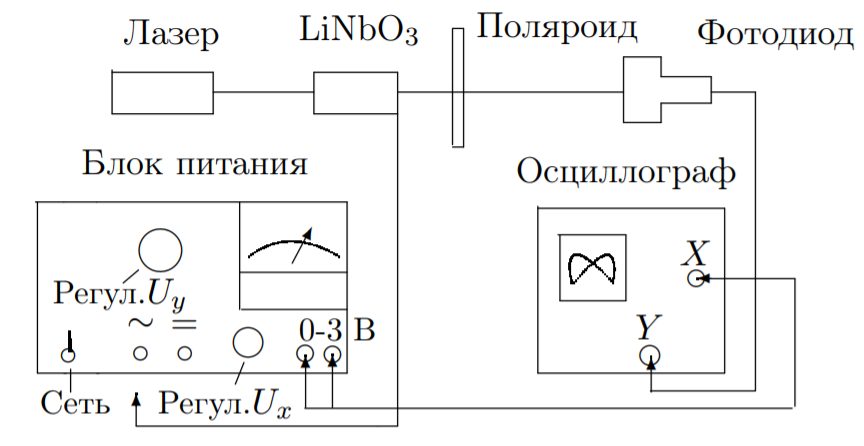
\includegraphics[width = 0.6\textwidth]{2.png}
\end{center}
\caption{Схема установки}
\label{scheme}
\end{figure}
На рис. \ref{scheme} представлена схема всей установки (оптическая часть изображена на рис. \ref{scheme_watch}). Свет лазера, проходя сквозь пластину, рассеивается и падает на двоякопреломляющий кристалл. На экране за поляроидом видна интерференционная картина. Убрав рассеивающую пластину и подавая на кристалл постоянное напряжение, можно величиной напряжения влиять на поляризацию луча, вышедшего из кристалла. Заменив экран фотодиодом и подав на кристалл переменное напряжение, можно исследовать поляризацию с помощью осциллографа.

\newpage

\section{Ход работы}
\subsection{Юстировка системы}

\begin{enumerate}
	\item Соберём оптическую схему согласно рис. \ref{scheme_watch}. Включим лазер и установим анализатор (без кристалла в схеме) так, чтобы лазерное излучение через него не проходило (скрещенные поляризации). Лазерный луч поляризован вертикально.

	\item Поставим кристалл и установим перед ним вплотную к кювете матовую пластинку. Расстояние от кристалла до экрана $L = 75$ см.

	\item Получим на экране интерференционную картину. Отклоняя кристалл с помощью юстировочного винта и поворачивая рейтер с кюветой вокруг вертикальной оси, добьемся совмещения центра коноскопической картины с положением луча на экране в отсутствие матовой пластинки. При повороте анализатора на $90^\circ$ коноскопическая картина меняется на негативную.

	\begin{figure}[h!]
		\begin{minipage}{0.5\textwidth}
			\center{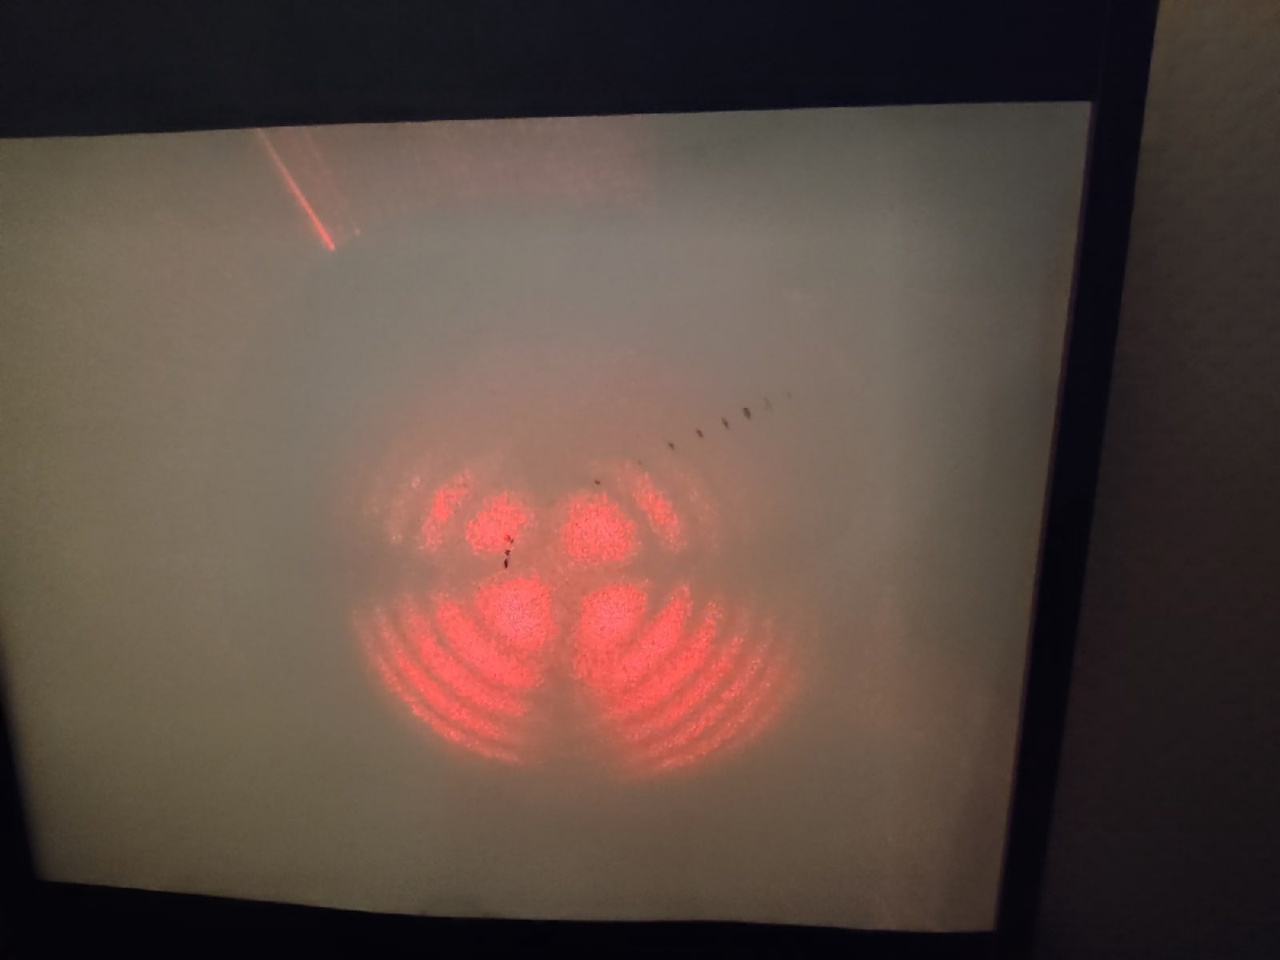
\includegraphics[width=1\textwidth]{interference.jpg} \\ а) Позитив}
		\end{minipage}
		\begin{minipage}{0.5\textwidth}
			\center{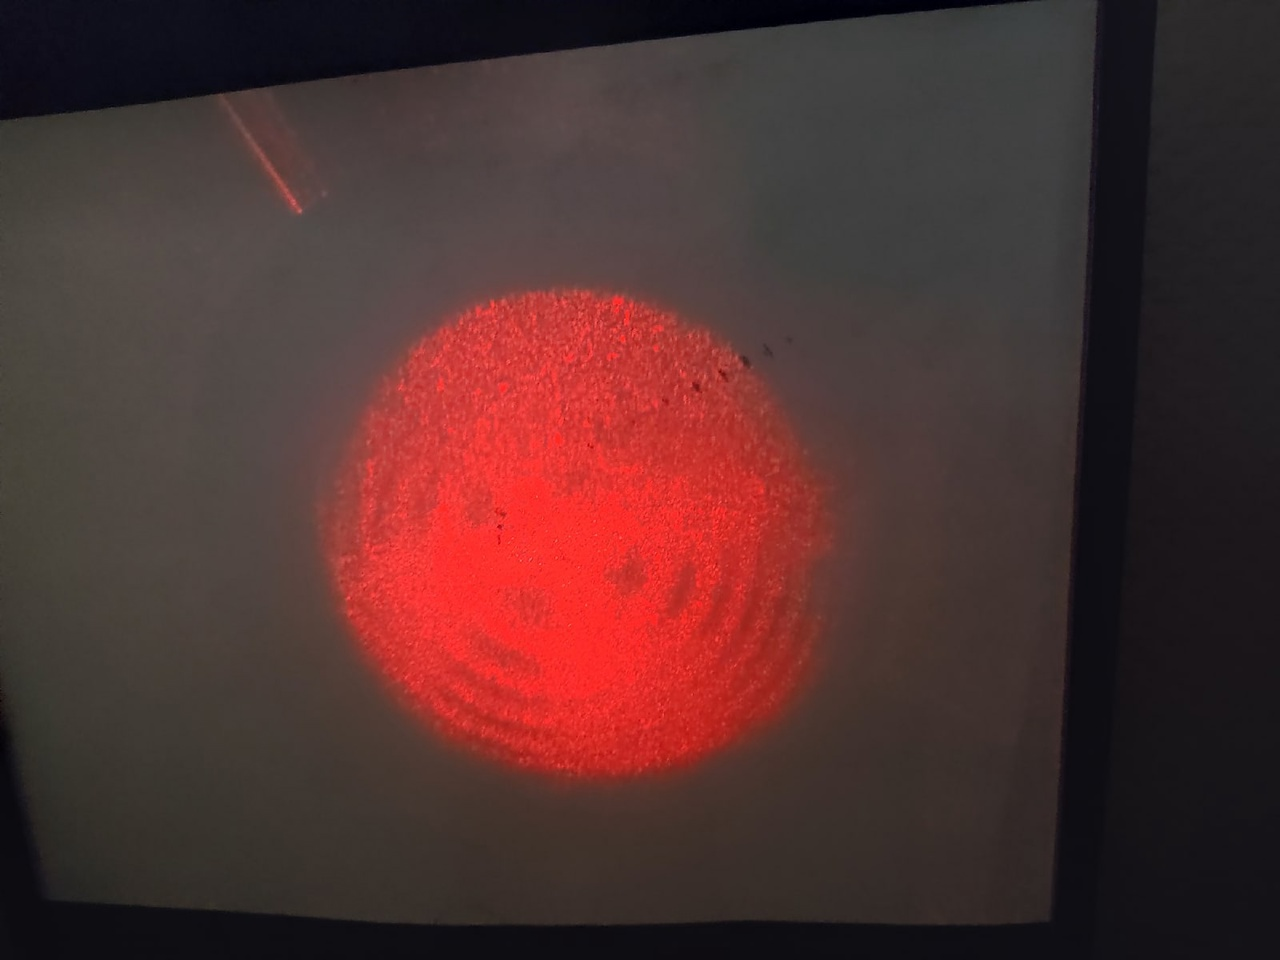
\includegraphics[width=1\textwidth]{interference_negative.jpg} \\ б) Негатив}
		\end{minipage}
		\caption{Интерференционная картина}
	\end{figure}
\end{enumerate}

\subsection{Измерения}

\begin{enumerate}
	\item Измерим радиусы тёмных колец и построим график $r^2 = f(m)$.

\clearpage
	\begin{table}[h!]
		\centering
		\begin{tabular}{|c|c|c|c|c|c|c|c|c|}
			\hline
			$m$                                           & 1      & 2     & 3     & 4     & 5  & 6     & 7  & 8     \\ \hline
			$r$, см                                       & 2,75   & 3,8   & 4,6   & 5,4   & 6  & 6,5   & 7  & 7,5   \\ \hline
			$r^2$, $см^2$ & 7,56 & 14,44 & 21,16 & 29,16 & 36 & 42,25 & 49 & 56,25 \\ \hline
			$\sigma_{r^2},~см^2$&0,28 &0,38 &0,46 &0,54 &0,60 &0,65 &0,70 &0,75 \\ \hline
		\end{tabular}
		\caption{Радиусы тёмных колец}
	\end{table}

\[\sigma_{r^2} = r^2\dfrac{\sigma_r}{r},~\sigma_r=1~{мм}\]
\[\sigma_k = \dfrac{1}{\sqrt{n}}\sqrt{\dfrac{<r^2m> - <r^2><m>}{<m^2> - <m>^2}}\]
\[\dfrac{\sigma_{n_o-n_e}}{n_o-n_e} = \sqrt{\left(\dfrac{\sigma_l}{l}\right)^2+2\left(\dfrac{\sigma_L}{L}\right)^2+\left(\dfrac{\sigma_k}{k}\right)^2}, ~\sigma_L=\sigma_l=1~{мм}\]


\begin{figure}[h!]
	\centering
	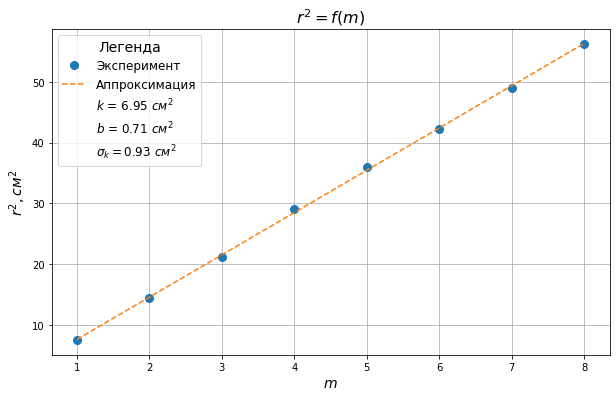
\includegraphics[width=1\textwidth]{graph1.png}
	\caption{Зависимость радиуса кольца от номера минимума}
	\label{Graph1}
\end{figure}

По углу наклона прямой определим двулучепреломление $(n_o-n_e)$ ниобата лития, пользуясь формулой (\ref{Radius_equation}); $\lambda =~$0,63 мкм, $L =~$75 см, $l =~$3 см (длина кристалла), $n_o =~$2,29:

\[n_o - n_e \approx \text{0,089}\pm\text{0,012}}\]

\item Уберём матовую пластинку и подключим разъём блока питания на постоянное напряжение (=), установим регулятор напряжения на минимальное напряжение и включим блок питания в сеть.

\begin{figure}[h!]
	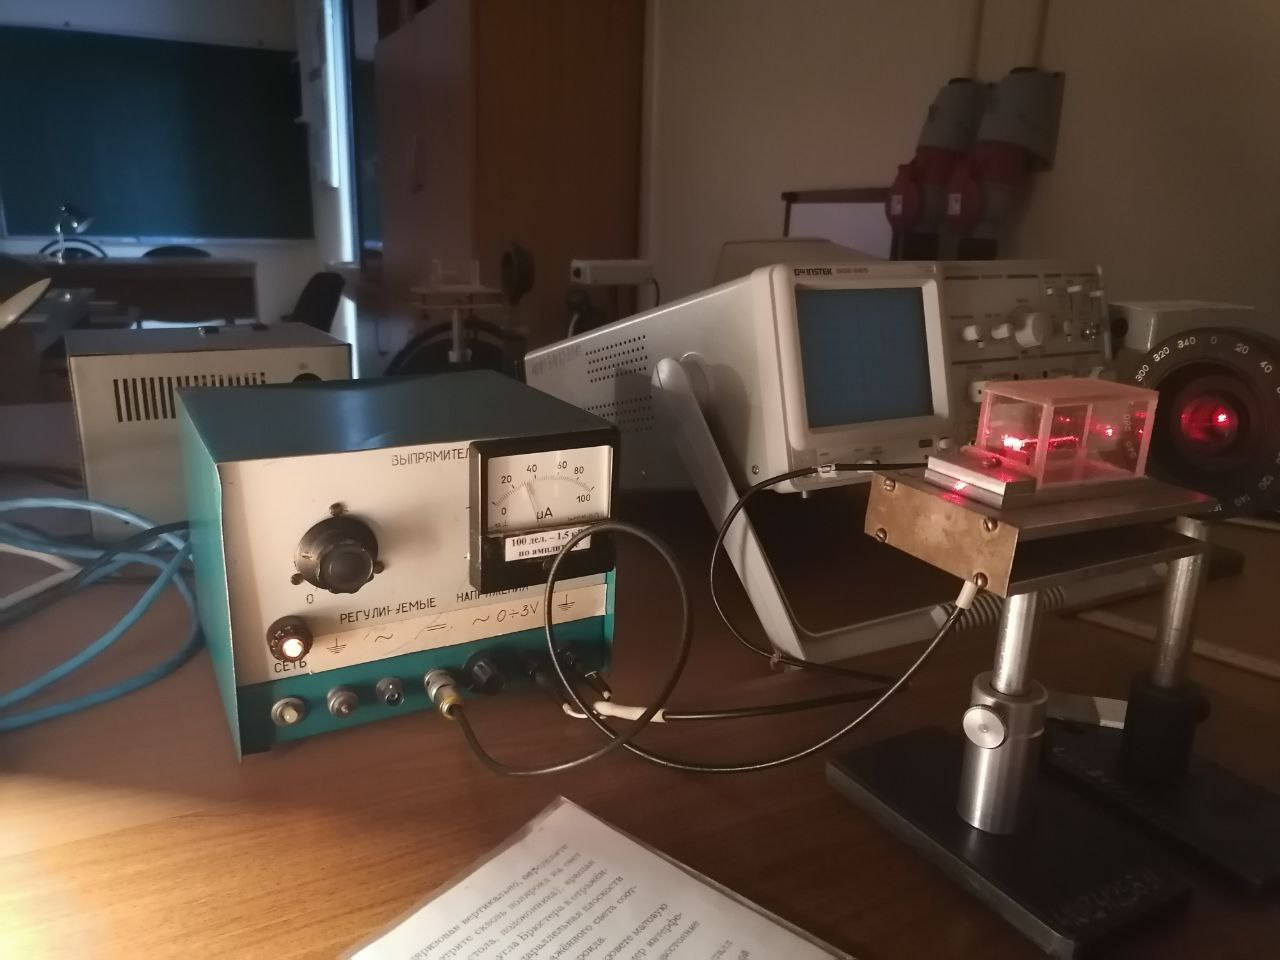
\includegraphics[width=1\textwidth]{Установка.jpg}
	\caption{Лабораторная установка}
	\label{Facility}
\end{figure}

Проследим, как меняется яркость пятна на экране с увеличением напряжения на кристалле.

Для скрещённых поляризаций при напряжениях $U = (2k-1)U_{\lambda/2}$ наблюдается максимум, при $U = 2kU_{\lambda/2}$ -- минимум, $k \in \mathbb{N}$. Для параллельных поляризаций наблюдается обратная зависимость.

В 100 делениях шкалы блока питания 1,5 кВ. Погрешность измерения напряжения 15 В.

\clearpage
\begin{table}[h!]
	\centering
	\begin{tabular}{|c|c|c|}
		\hline
                & Скрещённые поляризации & Параллельные поляризации \\ \hline
$U_{\lambda/2}$, В  & 570                    & 570                      \\ \hline
$U_{\lambda}$, В    & 1140                   & 1140                     \\ \hline
$U_{3\lambda/2}$, В & 1710                   & 1710                     \\ \hline
	\end{tabular}
	\caption{Напряжения, соответствующие экстремумам интенсивности, для двух видов поляризации}
\end{table}

\item Подадим на кристалл напряжение $U=\frac{1}{2}U_{\lambda/2}=U_{\lambda/4}=285\pm15$ В. При вращении анализатора наблюдаем малое изменение интенсивности пятна на экране, что доказывает наличие у луча на выходе из кристалла круговой поляризации.

\item Установим вместо экрана фотодиод и подключим его к $y$-входу осциллографа. Убрав напряжение до нуля, переключим разъём с постоянного (=) на переменное напряжение ($\sim$). С трёхвольтового выхода блока питания подадим сигнал на вход $x$ осциллографа. Отклонение луча осциллографа по оси $x$ пропорционально напряжению $U$ на кристалле, по оси $y$ -- интенсивности прошедшего через анализатор сигнала $I_{вых}$.

\item Постепенно повышая напряжение на кристалле, получим на экране осциллографа фигуры Лиссажу, соответствующие зависимости $I_{вых}(U)$ для скрещенных и параллельных поляризаций лазера и анализатора.

Определим по фигурам Лиссажу полуволновое напряжение, измерив разность показаний между последовательными фигурами, соответствующими максимуму и минимуму сигнала на осциллограме:
$\Delta U = U_{\lambda/2}\approx 570\pm15~В$.

\item Получим фигуры Лиссажу для напряжений $U_{\lambda/2}, U_{\lambda}, U_{3\lambda/2}}$ при скрещённых и параллельных поляризациях лазера и анализатора.

\clearpage
\begin{figure}[h!]
	\begin{minipage}{0.5\textwidth}
		\center{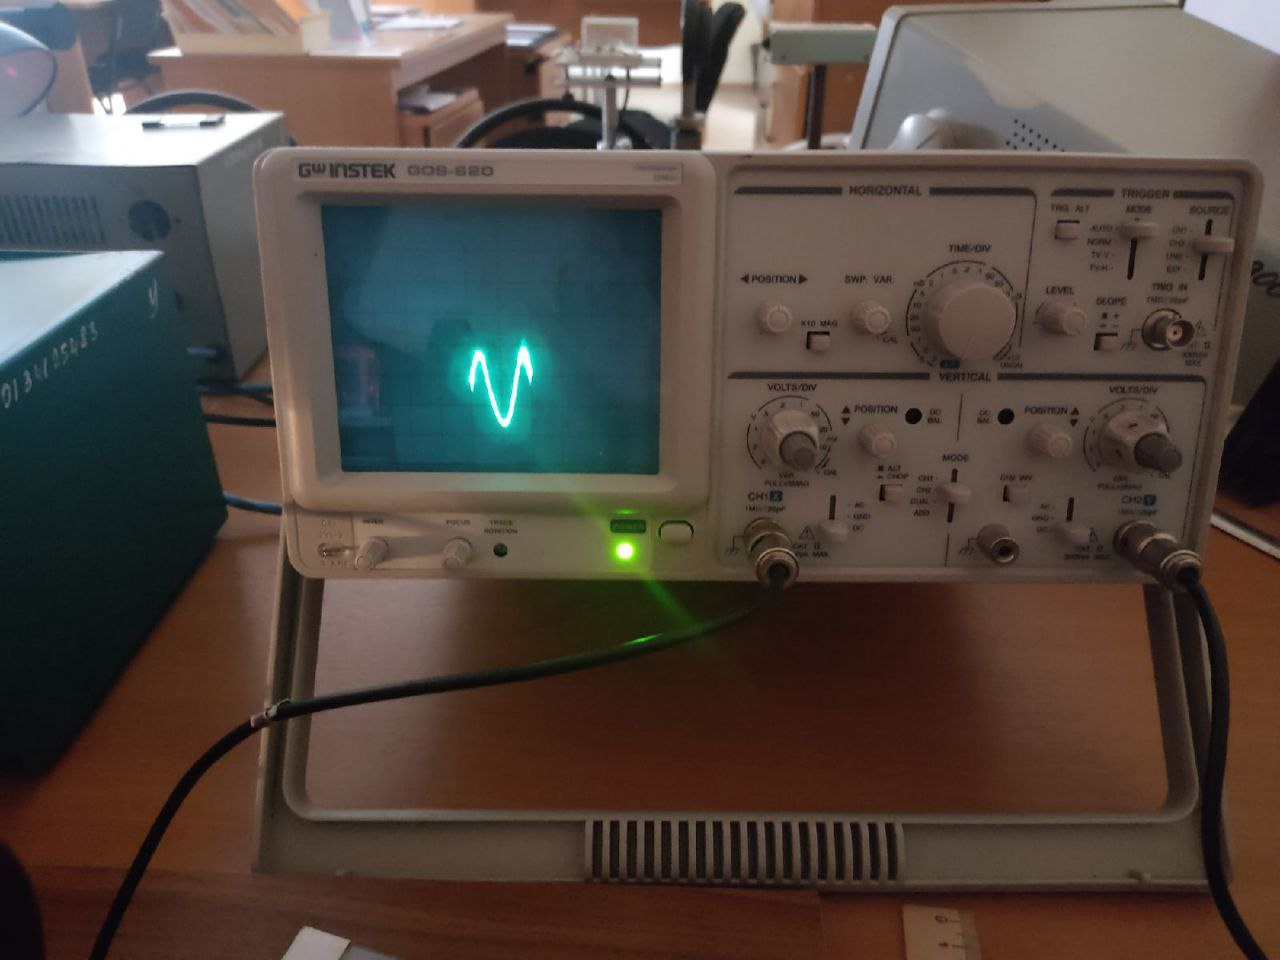
\includegraphics[width=1\textwidth]{Lissaju-3.jpg} \\ а) $U_{\lambda/2}$}
	\end{minipage}
	\begin{minipage}{0.5\textwidth}
		\center{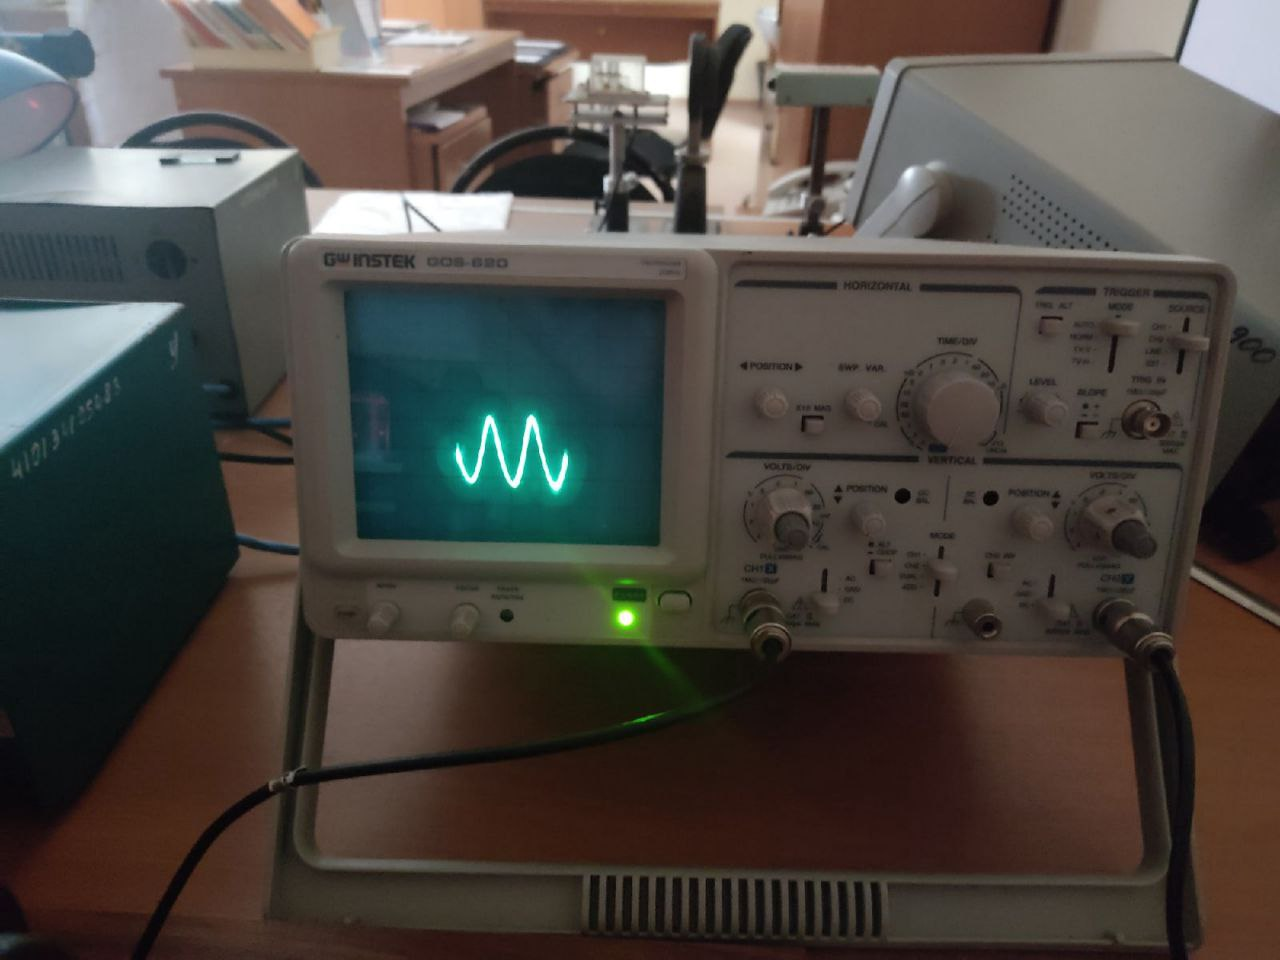
\includegraphics[width=1\textwidth]{Lissaju-2.jpg} \\ б) $U_{\lambda}$}
	\end{minipage}
	\begin{center}
	\begin{minipage}{0.5\textwidth}
		\center{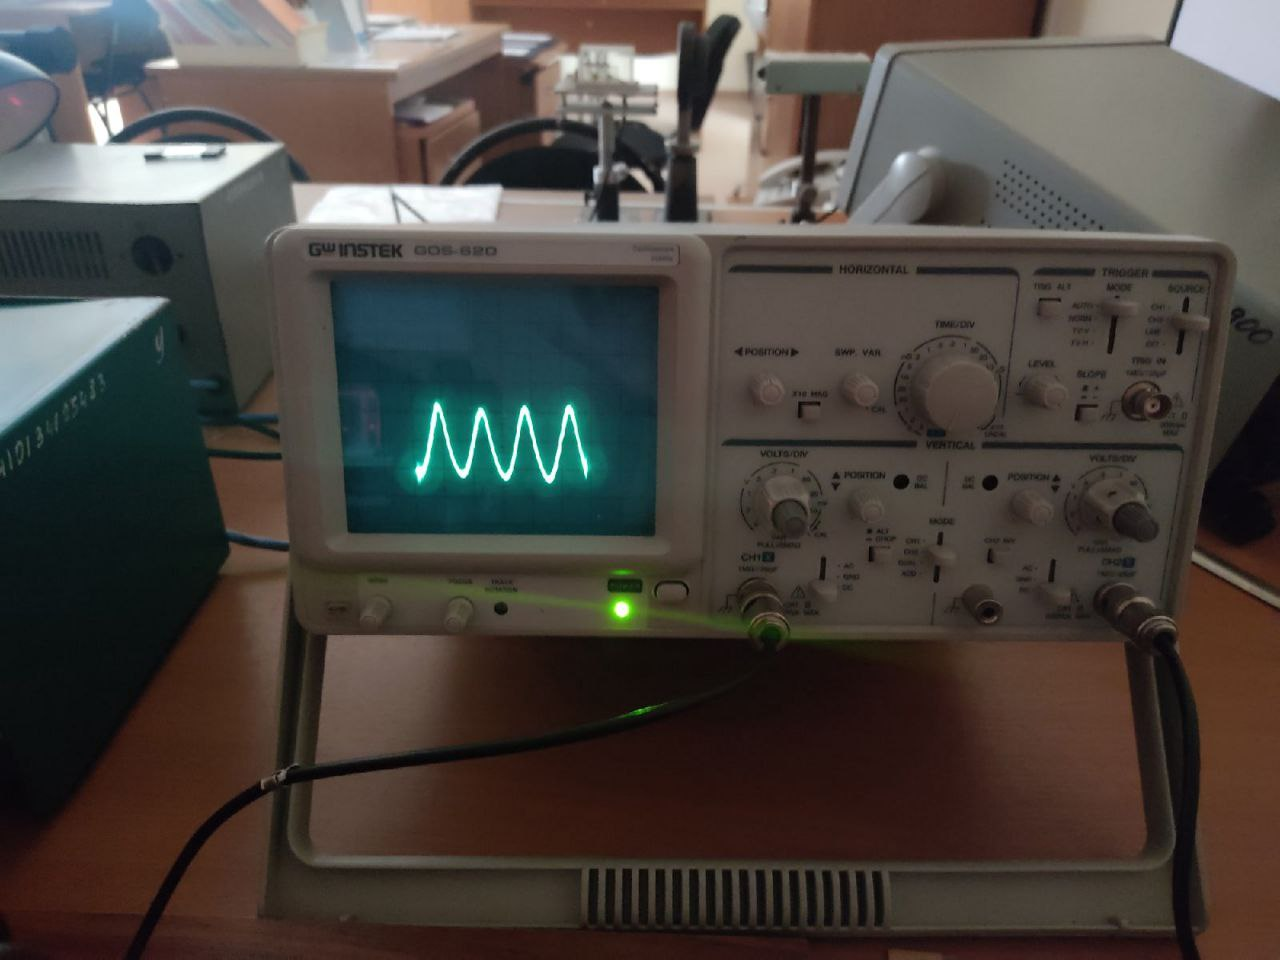
\includegraphics[width=1\textwidth]{Lissaju-1.jpg} \\ в) $U_{3\lambda/2}$}
	\end{minipage}
	\caption{Фигуры Лиссажу. Скрещённая поляризация}
	\end{center}
\end{figure}

\clearpage
\begin{figure}[h!]
	\centering
	\begin{minipage}{0.5\textwidth}
		\center{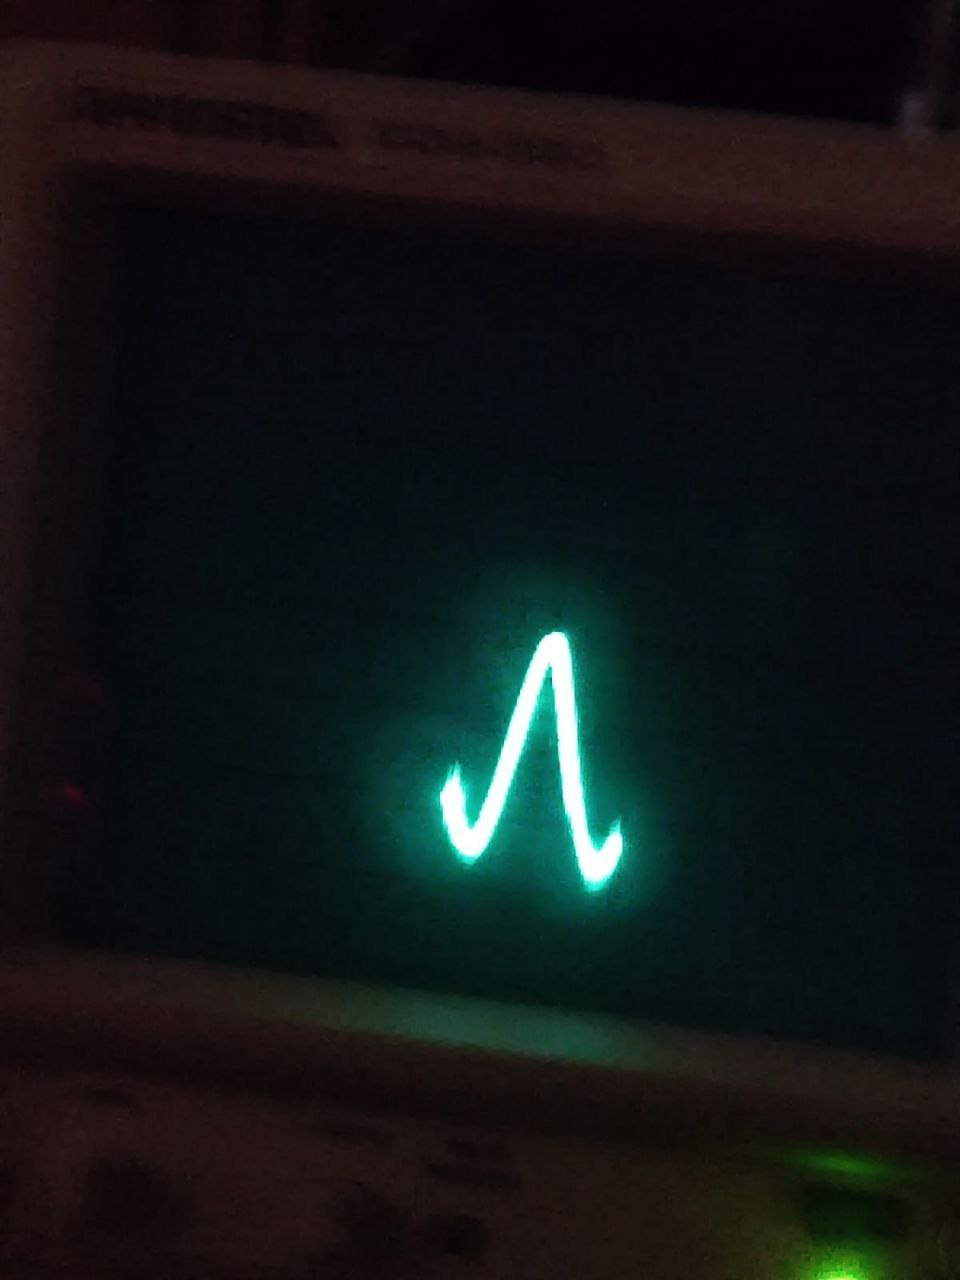
\includegraphics[width=0.75\textwidth]{Lissaju-3-par.jpg} \\ а) $U_{\lambda/2}$}
	\end{minipage}
	\begin{minipage}{0.5\textwidth}
		\center{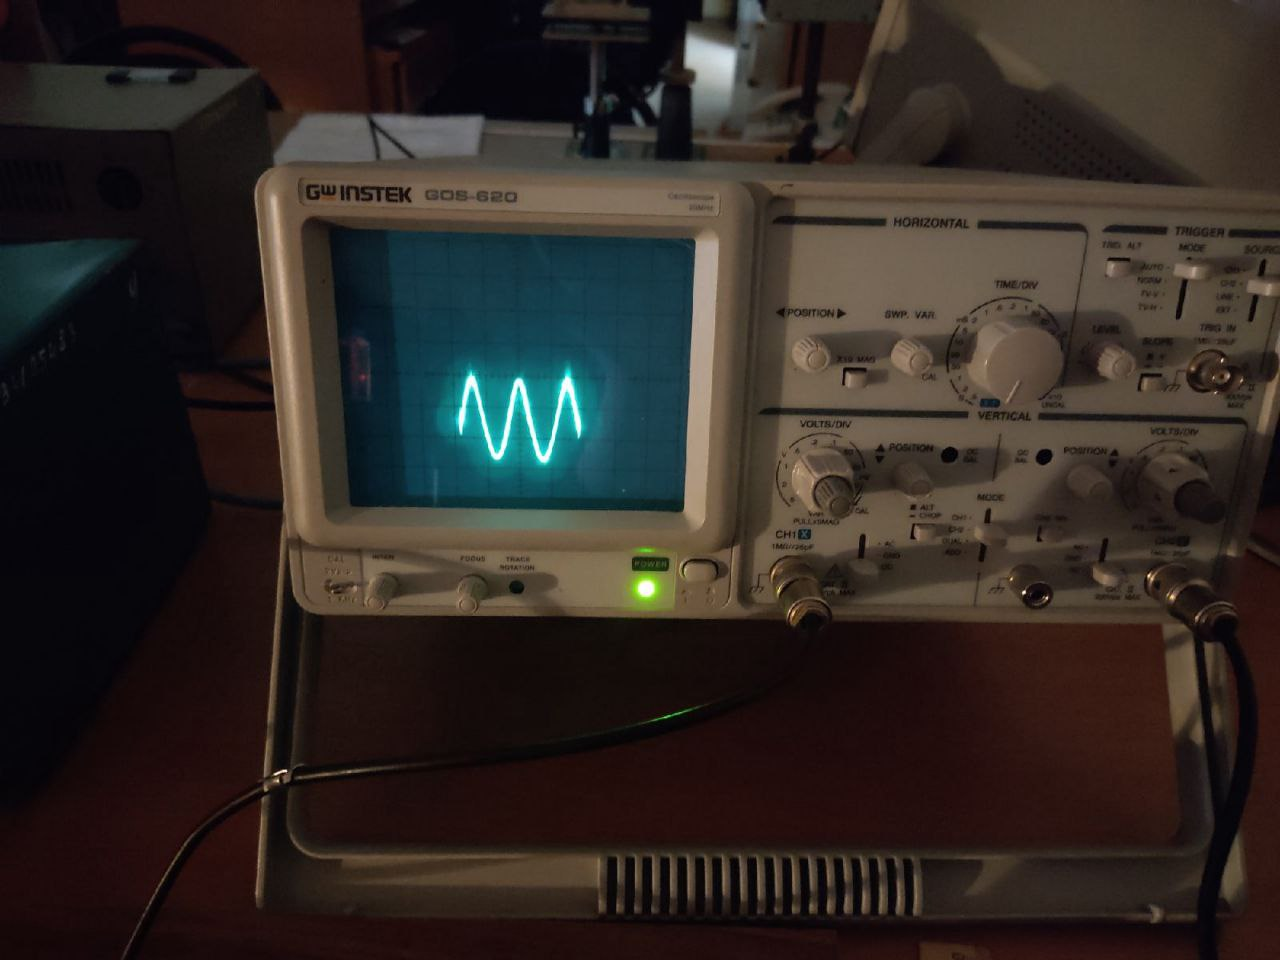
\includegraphics[width=1\textwidth]{Lissaju-2-par.jpg} \\ б) $U_{\lambda}$}
	\end{minipage}
	\begin{minipage}{0.5\textwidth}
		\center{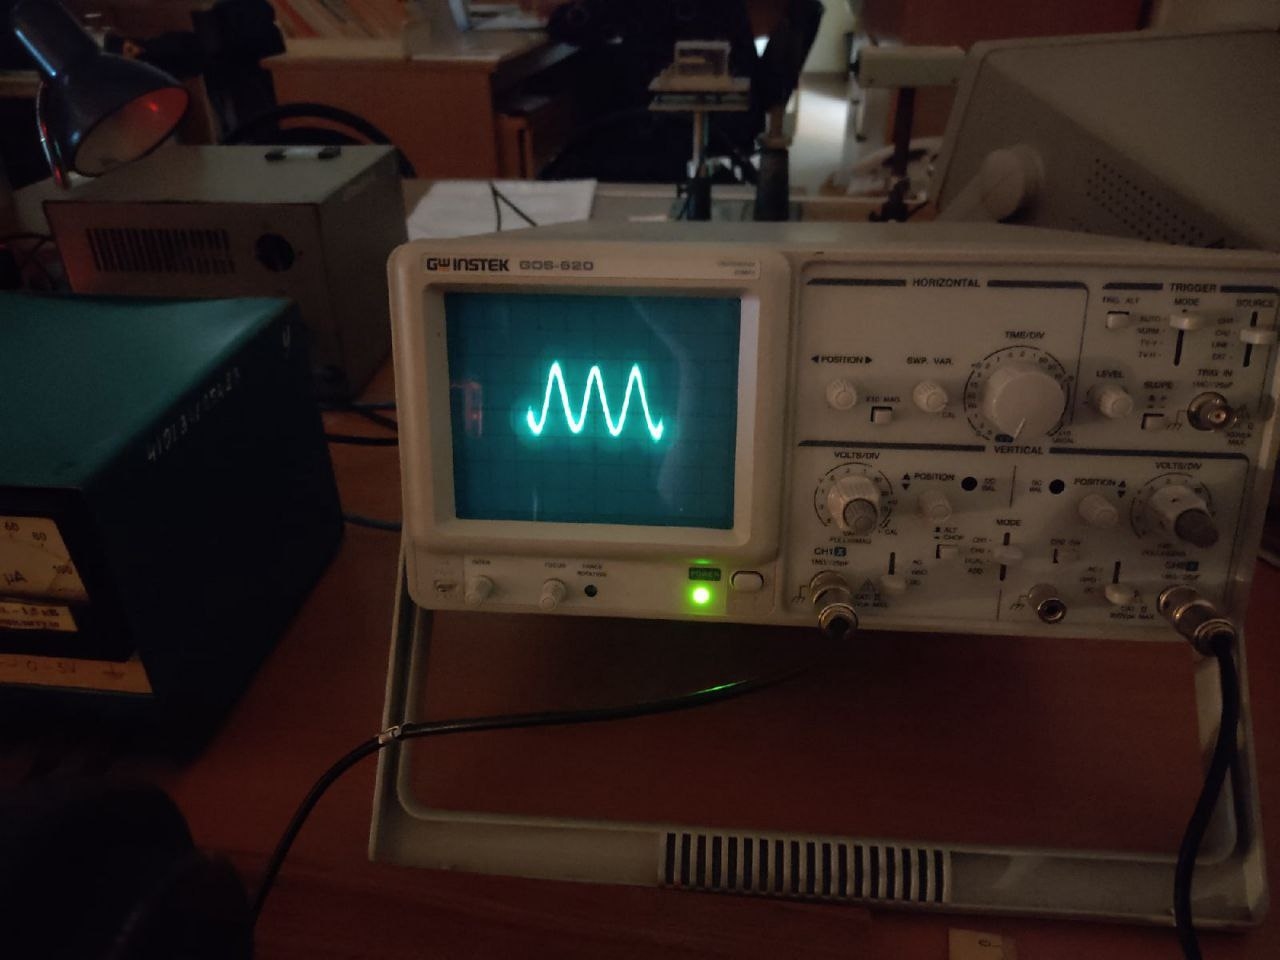
\includegraphics[width=1\textwidth]{Lissaju-1-par.jpg} \\ в) $U_{3\lambda/2}$}
	\end{minipage}
	\caption{Фигуры Лиссажу. Параллельная поляризация}
\end{figure}
\end{enumerate}

\section{Выводы}

\begin{enumerate}
	\item Была изучена интерференция рассеянного света, прошедшего кристалл ниобата лития;
	\item Были измерены радиусы $r_m$ интерференционных колец, определена разность показателей преломления $n_o-n_e = \text{0,089}\pm\text{0,012}$. Это значение соответствует литиевым кристаллам: $\Delta n \approx~$0,09;
	\item При подаче на кристалл постоянного напряжения $U_{\lambda/4}$ на выходе из кристалла был получен свет, поляризованный по кругу;
	\item Был исследован эффект Поккельса: двумя способами было получено полуволновое напряжение $U_{\lambda/2} \approx 570\pm15~В}$ (по зависимости интенсивности пятна на экране и по фигурам Лиссажу); по виду фигур Лиссажу установлено, что при скрещённых поляризациях лазера и анализатора $I_{вых}$ удовлетворяет формуле (\ref{I_sin}), при параллельных -- (\ref{I_cos}).
\end{enumerate}

\end{document}
